\begin{figure}
\centering
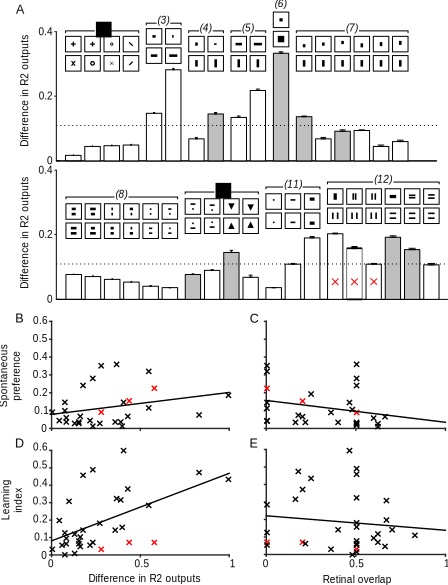
\includegraphics{figures/pattern}
\caption{How discriminable are different patterns for R2 neurons?
The bars indicate the \ac{rms} difference in activation for the R2 neurons when a pattern is at 0\textdegree\ and 90\textdegree.
A lower score indicates that the fly should find the pattern more difficult to discriminate.
Error bars show the standard error over the whole \ac{RIDF} (for examples see Figure~\ref{fig:recap}C--F).
The patterns are drawn from \protect\citeA{Ernst1999}; only patterns for which a statistical test was performed on the `differential conditioned preference' index (\overline{DCP}) are included.
Where a pattern was significantly learnable in \protect\citeA{Ernst1999}, the degree of significance is indicated by asterisks adjacent to the bars.
}
\label{fig:pattern}
\end{figure}
